% Options for packages loaded elsewhere
\PassOptionsToPackage{unicode}{hyperref}
\PassOptionsToPackage{hyphens}{url}
%
\documentclass[
  ignorenonframetext,
]{beamer}
\usepackage{pgfpages}
\setbeamertemplate{caption}[numbered]
\setbeamertemplate{caption label separator}{: }
\setbeamercolor{caption name}{fg=normal text.fg}
\beamertemplatenavigationsymbolsempty
% Prevent slide breaks in the middle of a paragraph
\widowpenalties 1 10000
\raggedbottom
\setbeamertemplate{part page}{
  \centering
  \begin{beamercolorbox}[sep=16pt,center]{part title}
    \usebeamerfont{part title}\insertpart\par
  \end{beamercolorbox}
}
\setbeamertemplate{section page}{
  \centering
  \begin{beamercolorbox}[sep=12pt,center]{part title}
    \usebeamerfont{section title}\insertsection\par
  \end{beamercolorbox}
}
\setbeamertemplate{subsection page}{
  \centering
  \begin{beamercolorbox}[sep=8pt,center]{part title}
    \usebeamerfont{subsection title}\insertsubsection\par
  \end{beamercolorbox}
}
\AtBeginPart{
  \frame{\partpage}
}
\AtBeginSection{
  \ifbibliography
  \else
    \frame{\sectionpage}
  \fi
}
\AtBeginSubsection{
  \frame{\subsectionpage}
}
\usepackage{amsmath,amssymb}
\usepackage{lmodern}
\usepackage{iftex}
\ifPDFTeX
  \usepackage[T1]{fontenc}
  \usepackage[utf8]{inputenc}
  \usepackage{textcomp} % provide euro and other symbols
\else % if luatex or xetex
  \usepackage{unicode-math}
  \defaultfontfeatures{Scale=MatchLowercase}
  \defaultfontfeatures[\rmfamily]{Ligatures=TeX,Scale=1}
\fi
\usetheme[]{AnnArbor}
\usecolortheme{dolphin}
\usefonttheme{structurebold}
% Use upquote if available, for straight quotes in verbatim environments
\IfFileExists{upquote.sty}{\usepackage{upquote}}{}
\IfFileExists{microtype.sty}{% use microtype if available
  \usepackage[]{microtype}
  \UseMicrotypeSet[protrusion]{basicmath} % disable protrusion for tt fonts
}{}
\makeatletter
\@ifundefined{KOMAClassName}{% if non-KOMA class
  \IfFileExists{parskip.sty}{%
    \usepackage{parskip}
  }{% else
    \setlength{\parindent}{0pt}
    \setlength{\parskip}{6pt plus 2pt minus 1pt}}
}{% if KOMA class
  \KOMAoptions{parskip=half}}
\makeatother
\usepackage{xcolor}
\newif\ifbibliography
\usepackage{color}
\usepackage{fancyvrb}
\newcommand{\VerbBar}{|}
\newcommand{\VERB}{\Verb[commandchars=\\\{\}]}
\DefineVerbatimEnvironment{Highlighting}{Verbatim}{commandchars=\\\{\}}
% Add ',fontsize=\small' for more characters per line
\usepackage{framed}
\definecolor{shadecolor}{RGB}{248,248,248}
\newenvironment{Shaded}{\begin{snugshade}}{\end{snugshade}}
\newcommand{\AlertTok}[1]{\textcolor[rgb]{0.94,0.16,0.16}{#1}}
\newcommand{\AnnotationTok}[1]{\textcolor[rgb]{0.56,0.35,0.01}{\textbf{\textit{#1}}}}
\newcommand{\AttributeTok}[1]{\textcolor[rgb]{0.77,0.63,0.00}{#1}}
\newcommand{\BaseNTok}[1]{\textcolor[rgb]{0.00,0.00,0.81}{#1}}
\newcommand{\BuiltInTok}[1]{#1}
\newcommand{\CharTok}[1]{\textcolor[rgb]{0.31,0.60,0.02}{#1}}
\newcommand{\CommentTok}[1]{\textcolor[rgb]{0.56,0.35,0.01}{\textit{#1}}}
\newcommand{\CommentVarTok}[1]{\textcolor[rgb]{0.56,0.35,0.01}{\textbf{\textit{#1}}}}
\newcommand{\ConstantTok}[1]{\textcolor[rgb]{0.00,0.00,0.00}{#1}}
\newcommand{\ControlFlowTok}[1]{\textcolor[rgb]{0.13,0.29,0.53}{\textbf{#1}}}
\newcommand{\DataTypeTok}[1]{\textcolor[rgb]{0.13,0.29,0.53}{#1}}
\newcommand{\DecValTok}[1]{\textcolor[rgb]{0.00,0.00,0.81}{#1}}
\newcommand{\DocumentationTok}[1]{\textcolor[rgb]{0.56,0.35,0.01}{\textbf{\textit{#1}}}}
\newcommand{\ErrorTok}[1]{\textcolor[rgb]{0.64,0.00,0.00}{\textbf{#1}}}
\newcommand{\ExtensionTok}[1]{#1}
\newcommand{\FloatTok}[1]{\textcolor[rgb]{0.00,0.00,0.81}{#1}}
\newcommand{\FunctionTok}[1]{\textcolor[rgb]{0.00,0.00,0.00}{#1}}
\newcommand{\ImportTok}[1]{#1}
\newcommand{\InformationTok}[1]{\textcolor[rgb]{0.56,0.35,0.01}{\textbf{\textit{#1}}}}
\newcommand{\KeywordTok}[1]{\textcolor[rgb]{0.13,0.29,0.53}{\textbf{#1}}}
\newcommand{\NormalTok}[1]{#1}
\newcommand{\OperatorTok}[1]{\textcolor[rgb]{0.81,0.36,0.00}{\textbf{#1}}}
\newcommand{\OtherTok}[1]{\textcolor[rgb]{0.56,0.35,0.01}{#1}}
\newcommand{\PreprocessorTok}[1]{\textcolor[rgb]{0.56,0.35,0.01}{\textit{#1}}}
\newcommand{\RegionMarkerTok}[1]{#1}
\newcommand{\SpecialCharTok}[1]{\textcolor[rgb]{0.00,0.00,0.00}{#1}}
\newcommand{\SpecialStringTok}[1]{\textcolor[rgb]{0.31,0.60,0.02}{#1}}
\newcommand{\StringTok}[1]{\textcolor[rgb]{0.31,0.60,0.02}{#1}}
\newcommand{\VariableTok}[1]{\textcolor[rgb]{0.00,0.00,0.00}{#1}}
\newcommand{\VerbatimStringTok}[1]{\textcolor[rgb]{0.31,0.60,0.02}{#1}}
\newcommand{\WarningTok}[1]{\textcolor[rgb]{0.56,0.35,0.01}{\textbf{\textit{#1}}}}
\usepackage{longtable,booktabs,array}
\usepackage{calc} % for calculating minipage widths
\usepackage{caption}
% Make caption package work with longtable
\makeatletter
\def\fnum@table{\tablename~\thetable}
\makeatother
\setlength{\emergencystretch}{3em} % prevent overfull lines
\providecommand{\tightlist}{%
  \setlength{\itemsep}{0pt}\setlength{\parskip}{0pt}}
\setcounter{secnumdepth}{-\maxdimen} % remove section numbering
\title[ VC55 Weather Case Study]{VC55 Long Term Weather Data From Sutton Bonnington} % The short title appears at the bottom of every slide, the full title is only on the title page
\subtitle{A case study using data state to analyse inconvenient data}

%\author{Dr. Paul J. Palmer}

\institute[LU] % Your institution as it will appear on the bottom of every slide, may be shorthand to save space
{
    Visiting Fellow \\
    Loughborough University \\
    \copyright~P.J.~Palmer~2022
    
    
    
    % Your institution for the title page
}
\author{}
\date{\vspace{-2.5em}\today} % Date, can be changed to a custom date

  %title: ""
 % author: Dr. Paul J. Palmer
  %date:  "`r format(Sys.time(), '%d %B, %Y')`"
\ifLuaTeX
  \usepackage{selnolig}  % disable illegal ligatures
\fi
\IfFileExists{bookmark.sty}{\usepackage{bookmark}}{\usepackage{hyperref}}
\IfFileExists{xurl.sty}{\usepackage{xurl}}{} % add URL line breaks if available
\urlstyle{same} % disable monospaced font for URLs
\hypersetup{
  pdftitle={VC55 Weather Case Study},
  pdfauthor={Paul J. Palmer},
  hidelinks,
  pdfcreator={LaTeX via pandoc}}

\title{VC55 Weather Case Study}
\author{Paul J. Palmer}
\date{}

\begin{document}
\frame{\titlepage}

\begin{frame}{Introduction}
\protect\hypertarget{introduction}{}
\begin{itemize}
\tightlist
\item
  The purpose of this vignette is a practical demonstration of reusable
  templates based upon the novel concept of data state.
\item
  This report is used as a case study for the paper: \emph{Achieving
  Analytical Fluency With Complex Data} and uses real world long term
  weather data as its source.
\item
  It is not the intention to analyse climate change, but the trends
  uncovered are striking, even in this single public domain source.
\end{itemize}
\end{frame}

\begin{frame}[fragile]{Load Libraries}
\protect\hypertarget{load-libraries}{}
\begin{Shaded}
\begin{Highlighting}[]
\FunctionTok{library}\NormalTok{(tidyverse) }\CommentTok{\# Load all the Tidyverse packages }
\CommentTok{\#in one go.}
\FunctionTok{library}\NormalTok{(kableExtra) }\CommentTok{\# Enable advanced table styling}
\FunctionTok{library}\NormalTok{(qqplotr) }\CommentTok{\# Enable QQ plots for statistical analysis}
\FunctionTok{library}\NormalTok{(readr) }\CommentTok{\# Improved reading of text files}
\FunctionTok{library}\NormalTok{(timeDate) }\CommentTok{\# Helper for time date manipulation}
\FunctionTok{library}\NormalTok{(rprojroot) }\CommentTok{\# Useful utilities}
\FunctionTok{library}\NormalTok{(fs) }\CommentTok{\# System independent file paths}
\end{Highlighting}
\end{Shaded}

Load the Tidyverse libraries and other helpers before the analysis
starts.
\end{frame}

\begin{frame}[fragile]{Read The Sutton Bonnington Data}
\protect\hypertarget{read-the-sutton-bonnington-data}{}
The source data is a text file that contains the following nominal data
fields in an inconvenient format: YYYY, mm, tmax.degC, tmin.degC,
airfrost.days, rain.mm, and sun.hours.

In addition we can also deduce the following fields using our
understanding of what the data represents in the real world: place.name,
latitude, longitude, height.amsl.metre

We use the function \texttt{get.weather.data.txt()} to encapsulate all
the actions necessary to achieve this in a way that is independent of
the actual data.

\begin{Shaded}
\begin{Highlighting}[]
\NormalTok{path.to.data }\OtherTok{\textless{}{-}}
\NormalTok{  fs}\SpecialCharTok{::}\FunctionTok{path}\NormalTok{(}\StringTok{"data{-}ext"}\NormalTok{, }\StringTok{"suttonboningtondata"}\NormalTok{, }\AttributeTok{ext =} \StringTok{"txt"}\NormalTok{)}
\NormalTok{suttonboningtondata }\OtherTok{\textless{}{-}} \FunctionTok{get.weather.data.txt}\NormalTok{(path.to.data)}
\end{Highlighting}
\end{Shaded}
\end{frame}

\begin{frame}[fragile]{Introducing Datum Triples}
\protect\hypertarget{introducing-datum-triples}{}
\begin{figure}

{\centering 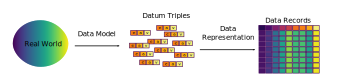
\includegraphics[width=0.7\linewidth]{images/standalone-data-definition} 

}

\caption{ Data representation}\label{fig:FigTheoryNascentData}
\end{figure}

The datum triple (Entity; Attribute; Value) is the universal starting
point for all data and requires the explicit use of a unique identifier
for each row which we call \texttt{datumEntity}. When data is in a wide
format, as at present, the identifier is implicit as in the row number,
but this is a relative term that is affected by order. Note that this
format makes no presumptions about number or types of attributes, and
implicitly casts all the data in character format . There is no reason
to keep any attribute with a value of \texttt{NA} as the row contains no
information.
\end{frame}

\begin{frame}[fragile]{File Contents}
\protect\hypertarget{file-contents}{}
The first 12 rows of the \texttt{weather.data.triple} now look like
this:

\begin{longtable}[]{@{}
  >{\centering\arraybackslash}p{(\columnwidth - 4\tabcolsep) * \real{0.3889}}
  >{\centering\arraybackslash}p{(\columnwidth - 4\tabcolsep) * \real{0.2778}}
  >{\centering\arraybackslash}p{(\columnwidth - 4\tabcolsep) * \real{0.1806}}@{}}
\toprule()
\begin{minipage}[b]{\linewidth}\centering
datumEntity
\end{minipage} & \begin{minipage}[b]{\linewidth}\centering
datumAttribute
\end{minipage} & \begin{minipage}[b]{\linewidth}\centering
datumValue
\end{minipage} \\
\midrule()
\endhead
Sutton.Bonnington:1959:01 & YYYY & 1959 \\
Sutton.Bonnington:1959:01 & mm & 01 \\
Sutton.Bonnington:1959:01 & tmax.degC & 4.2 \\
Sutton.Bonnington:1959:01 & tmin.degC & -2.4 \\
Sutton.Bonnington:1959:01 & airfrost.days & 23 \\
Sutton.Bonnington:1959:01 & sun.hours & 78.8 \\
Sutton.Bonnington:1959:01 & YYYYMMDD & 1959-01-31 \\
Sutton.Bonnington:1959:01 & lattitude & 52.833 \\
Sutton.Bonnington:1959:01 & longitude & -1.25 \\
Sutton.Bonnington:1959:01 & easting & 450700 \\
Sutton.Bonnington:1959:01 & northing & 325900 \\
Sutton.Bonnington:1959:01 & height.amsl.metre & 48 \\
\bottomrule()
\end{longtable}
\end{frame}

\begin{frame}[fragile]{Saving The Raw Data}
\protect\hypertarget{saving-the-raw-data}{}
Finally we can save the data in the datum triple format for reuse.
Although we have termed this as \texttt{data-raw}, multiple choices have
been made in its transformation into this state, so is it really raw
data? It should be clear that this \texttt{state} makes no assumptions
about the data fields in any observation, so multiple files can be saved
in the same directory as long as they use the same names for the three
columns in the datum triple.

\begin{Shaded}
\begin{Highlighting}[]
\FunctionTok{save.data.as.triple}\NormalTok{(suttonboningtondata,}\StringTok{"suttonboningtondata"}\NormalTok{)}
\end{Highlighting}
\end{Shaded}
\end{frame}

\begin{frame}[fragile]{Starting The Analysis With Data-Raw}
\protect\hypertarget{starting-the-analysis-with-data-raw}{}
For the purpose of this vignette we load the \texttt{data-raw} to
demonstrate the the analysis could start with multiple files using the
search style loading.

\begin{Shaded}
\begin{Highlighting}[]
\CommentTok{\# Load data{-}raw as datum triples}
\NormalTok{weather.data.triple }\OtherTok{\textless{}{-}} \FunctionTok{load.data.raw}\NormalTok{(}\StringTok{"data{-}raw"}\NormalTok{)}
\end{Highlighting}
\end{Shaded}
\end{frame}

\begin{frame}[fragile]{Prepare \texttt{data-sl}}
\protect\hypertarget{prepare-data-sl}{}
From the raw data we now prepare \texttt{data-sl} which is a loosely
defined format of convenience. All the attributes are in character
format, but may be in many different units. Re-arranging into a wider
format is helpful as it is more human readable and easier to analyse.

\begin{Shaded}
\begin{Highlighting}[]
\CommentTok{\# Prepare data{-}sl}
\CommentTok{\# First prepare the long data}
\NormalTok{VC55.weather.sl }\OtherTok{\textless{}{-}}\NormalTok{ weather.data.triple }\SpecialCharTok{\%\textgreater{}\%}
                  \FunctionTok{pivot\_wider}\NormalTok{(}
  \AttributeTok{id\_cols =}\NormalTok{ datumEntity,}
  \AttributeTok{names\_from =}\NormalTok{ datumAttribute,}
  \AttributeTok{values\_from =}\NormalTok{ datumValue)}
\end{Highlighting}
\end{Shaded}
\end{frame}

\begin{frame}[fragile]{Why Use Wide Format?}
\protect\hypertarget{why-use-wide-format}{}
In this example we are interested in the weather through time so we
select the columns of interest and make a long format with the date as
the key column. At this point we can also lose any columns that are not
required that may have been present if multiple sources of
\texttt{data-raw} were used.

This wide format gives great flexibility with analysis and works well
with a Grammar of Graphic (GoG) approach. This contrasts with the
temptation to produce a compact summary of data as one might use in a
spreadsheet analysis. The versatility of GoG will become apparent as we
proceed and see how all plots may be specified by changing the GoG
verbs.
\end{frame}

\begin{frame}[fragile]{Create Data-ss}
\protect\hypertarget{create-data-ss}{}
\begin{Shaded}
\begin{Highlighting}[]
\CommentTok{\# But we are interesting in plotting the data by date so}

\NormalTok{  VC55.weather.ss }\OtherTok{\textless{}{-}}\NormalTok{ VC55.weather.sl }\SpecialCharTok{\%\textgreater{}\%} 
    \FunctionTok{select}\NormalTok{(}\StringTok{"YYYYMMDD"}\NormalTok{, }
           \StringTok{"tmax.degC"}\NormalTok{,}
           \StringTok{"tmin.degC"}\NormalTok{,}
           \StringTok{"airfrost.days"}\NormalTok{, }
           \StringTok{"sun.hours"}\NormalTok{ ,}
           \StringTok{"rain.mm"}\NormalTok{)     }\SpecialCharTok{\%\textgreater{}\%}
            \FunctionTok{pivot\_longer}\NormalTok{(}\SpecialCharTok{!}\NormalTok{YYYYMMDD,}
                  \AttributeTok{names\_to =} \StringTok{"datumAttribute"}\NormalTok{, }
                  \AttributeTok{values\_to =} \StringTok{"datumValue"}\NormalTok{) }
\end{Highlighting}
\end{Shaded}
\end{frame}

\begin{frame}[fragile]{Specify Data types}
\protect\hypertarget{specify-data-types}{}
At this point we can specify data types as Date and numeric for
analysis.

\begin{Shaded}
\begin{Highlighting}[]
\CommentTok{\# Specify data types}
\NormalTok{VC55.weather.ss}\SpecialCharTok{$}\NormalTok{YYYYMMDD }\OtherTok{\textless{}{-}}  
\NormalTok{  VC55.weather.ss}\SpecialCharTok{$}\NormalTok{YYYYMMDD }\SpecialCharTok{\%\textgreater{}\%}\NormalTok{ as.Date}
\NormalTok{VC55.weather.ss}\SpecialCharTok{$}\NormalTok{datumValue }\OtherTok{\textless{}{-}} 
\NormalTok{  VC55.weather.ss}\SpecialCharTok{$}\NormalTok{datumValue }\SpecialCharTok{\%\textgreater{}\%} \FunctionTok{as.numeric}\NormalTok{()}
\end{Highlighting}
\end{Shaded}
\end{frame}

\begin{frame}[fragile]{Save Data-ss}
\protect\hypertarget{save-data-ss}{}
We can now save into \texttt{data-ss}.

\begin{Shaded}
\begin{Highlighting}[]
\FunctionTok{dir.create}\NormalTok{( }
\NormalTok{          fs}\SpecialCharTok{::}\FunctionTok{path}\NormalTok{( }
            \StringTok{"data{-}ss"}\NormalTok{ ),  }
            \AttributeTok{showWarnings =} \ConstantTok{FALSE}\NormalTok{,}
            \AttributeTok{recursive =} \ConstantTok{TRUE}\NormalTok{) }\CommentTok{\# Create the directory}
\CommentTok{\#And save.}
\NormalTok{path.to.save.ss}\OtherTok{\textless{}{-}}\NormalTok{ fs}\SpecialCharTok{::}\FunctionTok{path}\NormalTok{( }
                               \StringTok{"data{-}ss"}\NormalTok{,}\StringTok{"VC55.weather.ss"}\NormalTok{,}
                            \AttributeTok{ext =} \StringTok{"rds"}\NormalTok{)}
\FunctionTok{saveRDS}\NormalTok{(VC55.weather.ss, path.to.save.ss)}
\end{Highlighting}
\end{Shaded}
\end{frame}

\begin{frame}[fragile]{Why Save Data-ss?}
\protect\hypertarget{why-save-data-ss}{}
Once again the data may be loaded and the analysis start from this
point.In this example the production of \texttt{data-ss} is quick, but
for large an complex data we may wish to cache results for speedier
analysis.

Rather than load as a named file, we demonstrate how multiple files in
\texttt{data-ss} may be loaded and combined in a simple action. Since
\texttt{data-ss} are strictly defined each file may be `stacked' to
combine into a larger data-set.
\end{frame}

\begin{frame}[fragile]{Load Data-ss}
\protect\hypertarget{load-data-ss}{}
\begin{Shaded}
\begin{Highlighting}[]
\CommentTok{\# Load data{-}ss}
\NormalTok{path.to.data.ss }\OtherTok{\textless{}{-}}\NormalTok{ fs}\SpecialCharTok{::}\FunctionTok{path}\NormalTok{(}\StringTok{"data{-}ss"}\NormalTok{)}

\NormalTok{VC55.weather.ss }\OtherTok{\textless{}{-}} \FunctionTok{list.files}\NormalTok{(}
\NormalTok{  path.to.data.ss,}
  \AttributeTok{pattern =} \StringTok{".rds"}\NormalTok{, }\CommentTok{\# Make a suitable filter. }
  \CommentTok{\# Use the dot for a wildcard.}
  \AttributeTok{full.names =} \ConstantTok{TRUE}\NormalTok{,}
  \AttributeTok{recursive =} \ConstantTok{TRUE}\NormalTok{)  }\SpecialCharTok{\%\textgreater{}\%}
\NormalTok{  purrr}\SpecialCharTok{::}\FunctionTok{map\_df}\NormalTok{(readRDS) }
\end{Highlighting}
\end{Shaded}
\end{frame}

\begin{frame}[fragile]{Simple Check Plot}
\protect\hypertarget{simple-check-plot}{}
By faceting on \texttt{datumAttribute} we can produce a separate graph
for each attribute. While is shows we have data, each graph has
different units, so the scales do not make sense.

\begin{center}\includegraphics[width=0.7\linewidth]{Sutton_Bonnington_weather_files/figure-beamer/SimpleCheckPlot-1} \end{center}
\end{frame}

\begin{frame}{Q-Q Plot Z-score Compared To Normal Distribution}
\protect\hypertarget{q-q-plot-z-score-compared-to-normal-distribution}{}
Rather than 5 separate plots, if we use z-scores instead then each plot
is normalised against zero and the standard deviation we can plot all
the points on a common scale. The results seem to show that while a
normal distribution is a reasonable model, this is not the case for
extreme variances.

\begin{center}\includegraphics[width=0.7\linewidth]{Sutton_Bonnington_weather_files/figure-beamer/CheckingDataDistributionQQ-1} \end{center}
\end{frame}

\begin{frame}{Normalising With Z-scores}
\protect\hypertarget{normalising-with-z-scores}{}
Rather than 5 separate plots, if we use z-scores instead then each plot
is normalised against zero and the standard deviation we can plot all
the points on a common scale. However, the result is hard to interpret
because the variation between points is large.

\begin{center}\includegraphics[width=0.7\linewidth]{Sutton_Bonnington_weather_files/figure-beamer/PointsWithZScoreCode-1} \end{center}
\end{frame}

\begin{frame}{Trends in With Z-scores}
\protect\hypertarget{trends-in-with-z-scores}{}
However, if try to fit a local trend (Loess curve), then it is easier to
visualise trends.

\begin{center}\includegraphics[width=0.7\linewidth]{Sutton_Bonnington_weather_files/figure-beamer/NormalisingWithZScoreCode-1} \end{center}
\end{frame}

\begin{frame}{Assumptions}
\protect\hypertarget{assumptions}{}
Our assumption or a normal distribution is reasonably valid, but not
perfect. As we are looking at weather data, it might be nice to look at:
Annual Total Rainfall, Annual Air Frost days, Annual Maximum
Temperature, and Annual Minimum Temperature. Again GoG comes to the
rescue and we can quickly produce the following plots.
\end{frame}

\begin{frame}[fragile]{Weather Plots In Native Units}
\protect\hypertarget{weather-plots-in-native-units}{}
For convenience, the plot routine has been written as a function so we
can get all the plots quickly by reusing the code and just changing the
selection attribute.

\begin{Shaded}
\begin{Highlighting}[]
\NormalTok{ggfun }\OtherTok{\textless{}{-}} \ControlFlowTok{function}\NormalTok{(dat, nice.title)\{}
\NormalTok{  plot.output }\OtherTok{\textless{}{-}} \FunctionTok{ggplot}\NormalTok{(}\AttributeTok{data =}\NormalTok{ dat,}
                \FunctionTok{aes}\NormalTok{(}\AttributeTok{x =}\NormalTok{ YYYY,}
                    \AttributeTok{y =}\NormalTok{ annual)) }\SpecialCharTok{+}
    \FunctionTok{geom\_point}\NormalTok{() }\SpecialCharTok{+}
    \FunctionTok{geom\_smooth}\NormalTok{( }\AttributeTok{se =} \ConstantTok{FALSE}\NormalTok{, }
             \AttributeTok{method =} \StringTok{"lm"}\NormalTok{, }\AttributeTok{formula =} \StringTok{"y \textasciitilde{} x"}\NormalTok{) }\SpecialCharTok{+}
  \FunctionTok{geom\_line}\NormalTok{()}\SpecialCharTok{+} \FunctionTok{ggtitle}\NormalTok{( nice.title ) }\SpecialCharTok{+} \FunctionTok{ylab}\NormalTok{(nice.title)}
  \FunctionTok{return}\NormalTok{(plot.output)}
\NormalTok{\}}
\end{Highlighting}
\end{Shaded}
\end{frame}

\begin{frame}[fragile]{Filter The Data}
\protect\hypertarget{filter-the-data}{}
\begin{Shaded}
\begin{Highlighting}[]
\CommentTok{\# Weather "tmax.degC"     "tmin.degC"    }
\CommentTok{\# "airfrost.days" "sun.hours"     "rain.mm"}
\NormalTok{data.to.plot.local }\OtherTok{\textless{}{-}}\NormalTok{ VC55.weather.ss[}
\NormalTok{  VC55.weather.ss}\SpecialCharTok{$}\NormalTok{datumAttribute }\SpecialCharTok{==} \StringTok{"airfrost.days"}\NormalTok{, ]}
\NormalTok{data.to.plot.local}\SpecialCharTok{$}\NormalTok{YYYY }\OtherTok{\textless{}{-}} \FunctionTok{format}\NormalTok{(}
\NormalTok{  data.to.plot.local}\SpecialCharTok{$}\NormalTok{YYYYMMDD, }\AttributeTok{format =} \StringTok{"\%Y"}\NormalTok{) }\SpecialCharTok{\%\textgreater{}\%} 
    \FunctionTok{as.numeric}\NormalTok{()}
\NormalTok{data.to.plot.annual }\OtherTok{\textless{}{-}}\NormalTok{ data.to.plot.local }\SpecialCharTok{\%\textgreater{}\%} 
  \FunctionTok{drop\_na}\NormalTok{() }\SpecialCharTok{\%\textgreater{}\%} \FunctionTok{group\_by}\NormalTok{(YYYY) }\SpecialCharTok{\%\textgreater{}\%}
    \FunctionTok{mutate}\NormalTok{( }
  \CommentTok{\# Change to max, min etc. as required.}
          \AttributeTok{annual =} \FunctionTok{sum}\NormalTok{(datumValue)}
\NormalTok{        ) }
\end{Highlighting}
\end{Shaded}
\end{frame}

\begin{frame}{Plot Total Airfrost Days}
\protect\hypertarget{plot-total-airfrost-days}{}
\begin{center}\includegraphics[width=0.7\linewidth]{Sutton_Bonnington_weather_files/figure-beamer/PlotAirFrost-1} \end{center}
\end{frame}

\begin{frame}{Plot Maximum Temperature}
\protect\hypertarget{plot-maximum-temperature}{}
\begin{center}\includegraphics[width=0.7\linewidth]{Sutton_Bonnington_weather_files/figure-beamer/PlotMaxTemp-1} \end{center}
\end{frame}

\begin{frame}{Plot Minimum Temperature}
\protect\hypertarget{plot-minimum-temperature}{}
\begin{center}\includegraphics[width=0.7\linewidth]{Sutton_Bonnington_weather_files/figure-beamer/PlotMinTemp-1} \end{center}
\end{frame}

\begin{frame}{Plot Total Rainfail}
\protect\hypertarget{plot-total-rainfail}{}
\begin{center}\includegraphics[width=0.7\linewidth]{Sutton_Bonnington_weather_files/figure-beamer/PlotTotalRainfall-1} \end{center}
\end{frame}

\begin{frame}{Conclusion}
\protect\hypertarget{conclusion}{}
This vignette demonstrates the versatility of using data state in
conjunction with GoG.
\end{frame}

\end{document}
